\chapter{Future Work}
Overall the visualizations and prototypes represent a solid step towards a useful research tool for reconstructing MRI images. The work also provides a foothold for a number of potential future projects.

\section{Scan Simulation}
The scan simulation feature was received well on the whole however there is a long list of additional artefacts that could be added. With enough time they could all be included.

It does however raise the question of exactly how much realism is needed to effectively test a reconstruction algorithm? Highly realistic MRI simulation has been done before and tools, such as MRiLab\cite{mrilab}, allow the user to experiment with different scan sequences, coils and more. However, how far along this path we need to go to test reconstruction algorithm remains an area where more research is needed.

\section{Reconstruction}
My time spent with researchers indicated that overall they are willing to spend time labelling slice stacks, but only if they really need to, and only the minimum number required. Four landmarks is sufficient to define a rigid transformation (translation and rotation only) and this may prove sufficient for some scans, however the more deformable the organ, the more landmarks are required. The position of the landmarks is also important, having four  along the same axis is of no use, and how likely the landmark is to be obscured is also a consideration.

There are many efficiency savings that can be investigated to improve this step. One interesting approach would be to introduce the concept of iterated reconstruction: an initial reconstruction is first performed and then, based on the uncertainty that results the user can be prompted to provide landmarks in uncertain regions. This procedure can then be repeated, with only small parts of the volume requiring reconstruction at each step, until the uncertainty is at an acceptable level.

If the algorithm could also output the current best guess for each landmark this would also be beneficial. Moving the landmarking process from a completely manual "find all these landmarks" to a supervised "here are some landmarks - are they correct" approach will not just save time, but also be less tedious.

\section{Visualization}
The visualizations implemented provide a way of communicating the uncertainty in a manner far easier than looking at the raw data.

Originally the main aim of the project was to decide which of the two approaches to visualization was the best, then the winner could be further refined and used. If there had to be a winner then judging from the feedback it would have to be thresholding. When asked which they preferred 7 out of 9 said that thresholding was their favourite and only 2 preferred the surface representation.

Having said that it has been suggested that the surface representations did a good job of providing an overview, but to really understand the uncertainty it was necessary to delve into the details with thresholding. In that sense, perhaps the two types aren't competing with each other but provide different levels of detail.

Another important point to make is that it is just as important to show where the uncertainty is as it is to indicate why it became uncertain. The two visualizations both concentrate on the first point, which is useful to determine areas that should be avoided but doesn't explicitly tell you how to fix it. An interesting and potentially very useful extension would be to target individual types of uncertainty (see section \ref{background:uncertainty}) and develop specific visualizations. For example the sampling uncertainty (which indicates how much data there was to perform the reconstruction at that point) could be represented by overlaying the positions of the original stacks (after motion correction) on the reconstructed image.

One limitation of these visualizations is that they only really work with stationary targets, like the brain. An interesting point for future work would be to try and extend the visualizations to show how uncertainty in a cine (moving MRI image) changes over time. The use of time as a dimension available to visualize remained unexplored in this project, purely due to time constraints.

There is also a great deal of improvement to be had by adjusting the colours used. Currently the visualizations have a very simple 'colour' toggle that effectively changes the mapping from 'white to black' to 'black to red'. Colour was an area that was neglected in order to focus on ensuring the core functionality of the visualizations was solid.

The problem essentially boils down to the fact that there are 256 * 256 * 256 colours available and currently only 256 of them are being used. Changing this would be an easy fix and would instantly increase the contrast in all of the visualizations.

Each visualization also has a set of individual improvements that can be made to improve them:

\subsection*{Thresholding}
Currently the overlay is binary: it's either in the range or not. The possibility of extending this so that, within the threshold, higher uncertainty values standout more could be investigated. This could be done either by making values with higher uncertainty more opaque, or by investigating an alternate scheme, such as HSV (Hue, Saturation, Value). 

The hue and saturation (essentially the colour and how 'deep' it is) could be determined by the reconstructed scan and then the uncertainty could be mapped to the value (essentially how light it is). There are some issues that would need to be worked out with this approach, for example darker areas in the scan would likely appear more uncertain than light areas, even if they weren't.

\subsection*{Sphere}
The largest problem holding the sphere back was a lack of any reference point or anchoring in the scan. A number of suggestions to fix this were made including simply marking the top, bottom, left and right and also projecting common landmarks, such as the eyes, to the surface.

A more interactive approach could also be taken to solve this problem; a split screen visualization where the user could select a point in the reconstruction and the corresponding point on the sphere could be highlighted. Similarly if a point on the sphere was selected then the corresponding line could be highlighted in the volume.

The sphere was intended to be an abstract representation of the object, but in a sense it may be more abstract than is necessary. Many organs are roughly elliptical in shape and so one extension would be to allow the user to stretch the sphere to improve the fit to the object.

\subsection*{Surface}
The effectiveness of the surface visualization is highly dependant on the surface that is used. For the demonstration the surface was generated using the reconstruction mask which has a few rough edges impacting the clarity and appeal. The mask was primarily used as it foregoes the need for a complex registration step, which mapping a general model of the organ would require.

The next step for this visualization should be to investigate registering a general model of the organ to the volume. Landmarks provided in the reconstruction step should prove useful for this. This would be particularly useful when trying to compare two reconstructions side by side.

In particular, when reconstructing the fetal brain, because it changes so much over the course of the pregnancy a different model will be needed for each milestone. Research has been done to build atlases of the developing brain\cite{fetalatlas} and incorporating these volumes into the surface visualization would be a good starting point.

Limitations of the projection algorithm should also be considered. It is primarily designed for visualizing large, convex objects. This is true for a large number of organs but when it comes to visualizing something small, like blood vessels, modifications may be required. For example the viewer is unlikely to want to have to trace along every vein, rotating around to see the uncertainty. Instead the uncertainty in an entire cross section should be mapped to the surface to give an overview.

\subsection*{Next Scan Plane}
The main hurdle to implementing this visualization is that the reconstruction process is not optimized enough to run in real time. This means that the uncertainty is not currently known at the time of scanning and further work needs to be done before this can be achieved.

This isn't the only hurdle that needs to be overcome; the radiographers are already under massive time pressures in the scan without them having to guide a reconstruction as well. The time available to complete the scanning is usually no more than 45-60 minutes which includes the time to set up and settle in the patient. Taking this into account either an extra person will be required to guide the reconstruction (masks, landmarking etc.) or much further automation is required.

% ------------------------- %
% ------- Labelling ------- %
% ------------------------- %
\newpage
\section{Labelling}\label{background:labelling}
One part of the project that there wasn't time to explore but would come in useful for further developments is labelling. Work on choosing a good labelling system has been done previously and there are a number of different approaches that can be taken\cite{labelling}.

For future work it will almost certainly be worth researching these techniques. See Figure~\ref{fig:labels} for examples.

\begin{figure}[H]
    \centering
	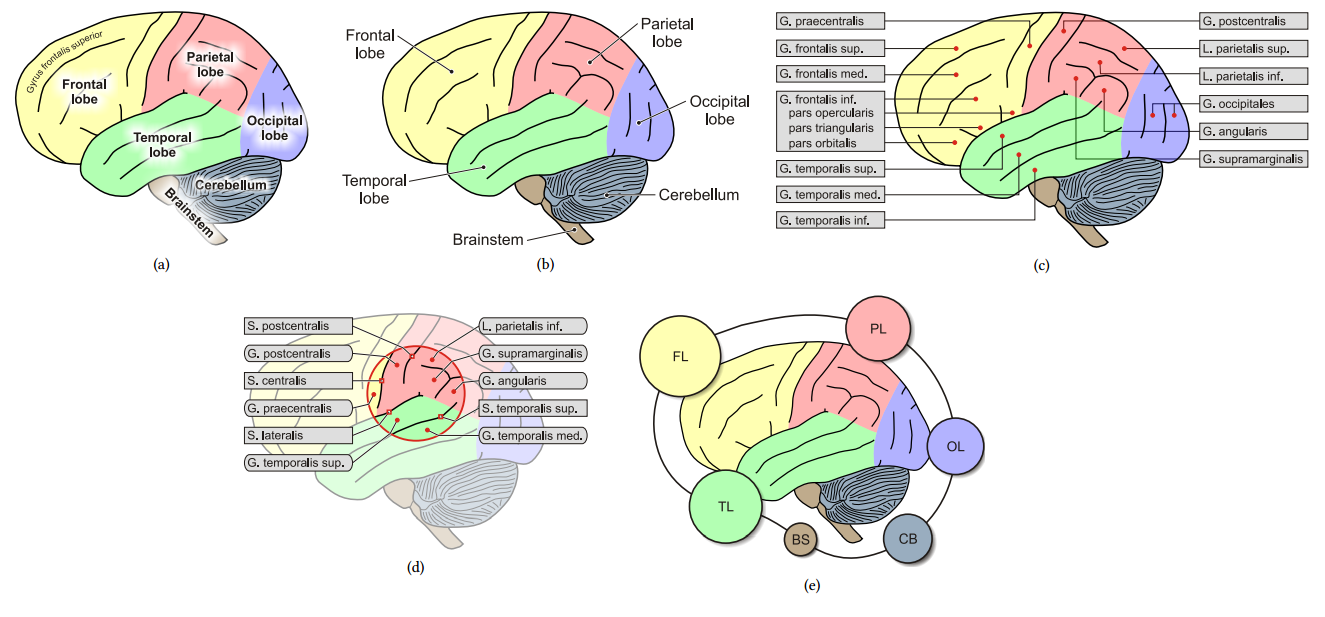
\includegraphics[width=1.0\textwidth]{images/background/labels.png}
    \caption{Different labelling techniques. Adapted from \cite{labelling}}
    \label{fig:labels}
\end{figure}